\documentclass{article}

% Language setting
% Replace `english' with e.g. `spanish' to change the document language
\usepackage[english]{babel}

% Set page size and margins
% Replace `letterpaper' with`a4paper' for UK/EU standard size
\usepackage[letterpaper,top=2cm,bottom=2cm,left=3cm,right=3cm,marginparwidth=1.75cm]{geometry}

% Useful packages
\usepackage{amsmath}
\usepackage{amsfonts}
\usepackage{amsthm}
\usepackage{graphicx}
\usepackage[colorlinks=true, allcolors=blue]{hyperref}

\title{Solutions - Quantum communication WS20/21}
\author{Christian Thierfelder}

\begin{document}
\maketitle


\section*{Problem Set 1}
    Quick recap - polarizing beam splitter
    \begin{center}
        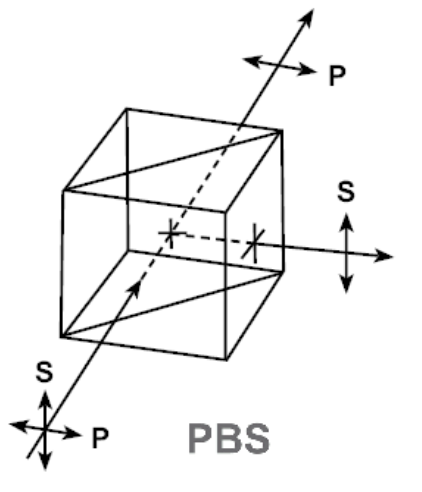
\includegraphics[width=0.25\textwidth]{PBS.png}
    \end{center}
    
    \begin{itemize}
        \item s-polarized - light whose electric field is normal to the plane of incidence
        \item p-polarized - polarized light with its electric field along the plane of incidence
    \end{itemize}
\begin{enumerate}
    \item
    \begin{enumerate}
        \item We assume $|H\rangle$=p-polarized and $|V\rangle$=s-polarized as well as $\langle V|H\rangle=0$. Then we use the Jones vector
        \begin{align}
            |\theta\rangle&=\begin{pmatrix}
            \cos\theta\\
            \sin\theta
            \end{pmatrix}\\
            |\theta'\rangle&=\begin{pmatrix}
            1 & 0\\
            0 & 0
            \end{pmatrix}
            \begin{pmatrix}
            \cos\theta\\
            \sin\theta
            \end{pmatrix}=
            \begin{pmatrix}
            \cos\theta\\
            0
            \end{pmatrix}
        \end{align}
        and obtain
        \begin{align}
            \text{transmitted}&\quad\rightarrow\quad |\langle H|\theta'\rangle|^2=\cos^2\theta\\
            \text{reflected}&\quad\rightarrow\quad \sin^2\theta
        \end{align}
        \item It is s-polarized so $cos\theta|H\rangle$
        \item See table
        \begin{table}[!h]
            \centering
            \begin{tabular}{c|c|c}
             $\theta$ & prob. reflected & prob. transmitted  \\
             \hline
             0         & 0 & 1\\
             $\pi/2$   & 1 & 0\\
             $\pi$     & 0 & 1\\
             $3\pi/2$  & 1 & 0\\
             $2\pi$    & 0 & 1\\
            \end{tabular}
            \caption{Probabilities for 1(c)}
            \label{tab:my_label}
        \end{table}
        \item With the rotated matrix ($\alpha=\pi/4$ and we forget about $-\pi/4$)
        \begin{align}
            \begin{pmatrix}
            \cos\alpha & -\sin\alpha\\
            \sin\alpha & \cos\alpha
            \end{pmatrix}
            \begin{pmatrix}
            1 & 0\\
            0 & 0
            \end{pmatrix}
            \begin{pmatrix}
            \cos\alpha & -\sin\alpha\\
            \sin\alpha & \cos\alpha
            \end{pmatrix}=\frac{1}{2}\begin{pmatrix}
            1 & 1\\
            1 & 1
            \end{pmatrix}
        \end{align}
        we have
        \begin{align}
            |\theta'\rangle&=\frac{1}{2}\begin{pmatrix}
            1 & 1\\
            1 & 1
            \end{pmatrix}
            \begin{pmatrix}
            \cos\theta\\
            \sin\theta
            \end{pmatrix}=
            \frac{1}{2}\begin{pmatrix}
            \cos\theta+\sin\theta\\
            \cos\theta+\sin\theta
            \end{pmatrix}
        \end{align}
        and obtain
        \begin{align}
            \text{transmitted}&\quad\rightarrow\quad |\langle H|\theta'\rangle|^2=\frac{1}{4}(\sin\theta+\cos\theta)^2=\frac{1}{4}(1+\sin2\theta)\\
            \text{reflected}&\quad\rightarrow\quad \frac{1}{4}(3-\sin2\theta)
        \end{align}
        \item It is $\frac{1}{2}(\sin\theta+\cos\theta)(|H\rangle+|V\rangle)$
        \item See table
        \begin{table}[!h]
            \centering
            \begin{tabular}{c|c|c}
             $\theta$ & prob. reflected & prob. transmitted  \\
             \hline
             $3\pi/4$   & 1 & 0\\
             $7\pi/4$   & 1 & 0
            \end{tabular}
            \caption{Probabilities for 1(f)}
            \label{tab:my_label}
        \end{table}
        \item With the phase shift matrix
        \begin{align}
            P=\begin{pmatrix}
            1 & 0\\
            0 & e^{i\varphi}
            \end{pmatrix}
        \end{align} 
        we have
        \begin{align}
        |\theta'\rangle=
        \begin{pmatrix}
            1 & 0\\
            0 & 0
            \end{pmatrix}
            \begin{pmatrix}
            1 & 0\\
            0 & e^{i\varphi}
            \end{pmatrix}
            \begin{pmatrix}
            \cos\theta\\
            \sin\theta
            \end{pmatrix}=
            \begin{pmatrix}
            \cos\theta\\
            0
            \end{pmatrix}
        \end{align} 
        so no change to the original result - transmission is $|\langle H|\theta'\rangle|^2=\cos^2\theta$ and reflection $\sin^2\theta$.
        \item Now we have
        \begin{align}
        |\theta'\rangle=
        \frac{1}{2}
        \begin{pmatrix}
            1 & 1\\
            1 & 1
            \end{pmatrix}
            \begin{pmatrix}
            1 & 0\\
            0 & e^{i\varphi}
            \end{pmatrix}
            \begin{pmatrix}
            \cos\theta\\
            \sin\theta
            \end{pmatrix}=\frac{1}{2}
            \begin{pmatrix}
            \cos\theta+e^{i\varphi}\sin\theta\\
            \cos\theta+e^{i\varphi}\sin\theta
            \end{pmatrix}
        \end{align} 
    so transmission is
    \begin{align}
        |\langle H|\theta'\rangle|^2=\frac{1}{4}(1+\cos\varphi\sin2\theta)
    \end{align}
    and reflection $\frac{1}{4}(3-\cos\varphi\sin2\theta)$
    \end{enumerate}
\end{enumerate}


\section*{Problem Set 2}
\begin{enumerate}
    \item 
    \begin{enumerate}
        \item To be an observable the operators must be hermitian ($A=A^\dagger$)  which means the eigenvalues are real - therefore 
        \begin{align}
            A|\psi_2\rangle=a_2|\psi_2\rangle\quad\rightarrow\quad \langle\psi_1|A|\psi_2\rangle=a_2\langle\psi_1|\psi_2\rangle\\
            \langle\psi_1|A=a_1\langle\psi_1|\quad\rightarrow\quad \langle\psi_1|A|\psi_2\rangle=a_1\langle\psi_1|\psi_2\rangle
        \end{align}
        in the non-degenerate ($a_1\ne a_2$ ) the result follows (and the same for $B$). In the degenerate case you always can orthogonalise the eigenstates but you don't have to!.
    
    \item For a pure state $|\varphi\rangle=c_1|\psi_1\rangle+c_2|\psi_2\rangle$ we have with $\mathbb{I}=\sum_k|\psi_k\rangle\langle\psi_k|$
    \begin{align}
        A|\varphi\rangle=\sum_ka_k|\psi_k\rangle\langle\psi_k|\varphi\rangle
    \end{align}
    The measurement of $A$ then filters out one eigenstate $|\psi_n\rangle$ with probability $|\langle\psi_n|\varphi\rangle|^2$ and the value $a_n$ is measured.
    \begin{align}
        \langle\psi_n|\varphi\rangle
        &=c_1\langle\psi_n|\psi_1\rangle+c_2\langle\psi_n|\psi_2\rangle\\
        &=c_n\langle\psi_n|\psi_n\rangle
    \end{align}
    If we assume(!) that the eigenstates were normalized then we obtain
    \begin{table}[!h]
        \centering
        \begin{tabular}{|c|c|c|}
        \hline
            value & state & probability\\
            \hline\hline
            $a_1$ & $|\psi_1\rangle$ & $|c_1|^2$ \\ \hline
            $a_2$ & $|\psi_2\rangle$ & $1-|c_1|^2$\\
            \hline
        \end{tabular}
        \caption{Measuring $A$}
        \label{tab:my_label}
    \end{table}
    
    For a mixed state with the density operator $\rho=\sum_ip_i|\phi_i\rangle\langle\phi_i|$ we obtain for the result of a measurement
    \begin{align}
        \langle A\rangle&=\text{tr}(A\rho)\\
        &=\sum_iA_{ki}\rho_{im}\\
        &=\sum_ip_i\langle\phi_i|A|\phi_i\rangle\\
        &=\sum_i\sum_{n,m}p_i\langle\phi_i|\varphi_m\rangle\langle\varphi_m|A|\varphi_n\rangle\langle\varphi_n|\phi_i\rangle\\
        &=\sum_i\sum_{n,m}p_i\langle\phi_i|\varphi_m\rangle A_{mn}\langle\varphi_n|\phi_i\rangle
    \end{align}
    for this special case we have
    \begin{align}
        \langle A\rangle
        &=\sum_i\sum_{n,m}p_i\delta_{mn}a_n\langle\phi_i|\psi_m\rangle \langle\psi_n|\phi_i\rangle\\
        &=\sum_i\sum_{m}p_ia_m|\langle\phi_i|\psi_m\rangle|^2.
    \end{align}
    
    \item We consider now that we started with a pure state (which resulted from the first measurement of $A$) - measuring $B$ results in \{$b_1$,$|\phi_1\rangle$\} or \{$b_2$,$|\phi_2\rangle$\}. For the probabilities we need to take the result of the first $A$ measurement into account
    \begin{itemize}
        \item $a_1$ was measured and system is in state $|\psi_1\rangle$ then
        \begin{align}
            |\langle\phi_1|\psi_1\rangle|^2&=\frac{9}{25}\\
            |\langle\phi_2|\psi_1\rangle|^2&=\frac{16}{25}
        \end{align}
        
        \item $a_2$ was measured and system is in state $|\psi_2\rangle$ then
        \begin{align}
            |\langle\phi_1|\psi_2\rangle|^2&=\frac{16}{25}\\
            |\langle\phi_2|\psi_2\rangle|^2&=\frac{9}{25}
        \end{align}
    \end{itemize}
    Then we can calculate the total probabilities via Bayes theorem
    \begin{align}
        P(A,B=b_1)
        &=P(B=b_1|A=a_1)P(A=a_1)+P(B=b_1|A=a_2)P(A=a_2)\\
        &=\frac{9}{25}|c_1|^2+\frac{16}{25}(1-|c_1|^2)\\
        &=\frac{16}{25}-\frac{7}{25}|c_1|^2\\
        P(A,B=b_2)
        &=P(B=b_2|A=a_1)P(A=a_1)+P(B=b_2|A=a_2)P(A=a_2)\\
        &=\frac{16}{25}|c_1|^2+\frac{9}{25}(1-|c_1|^2)\\
        &=\frac{9}{25}+\frac{7}{25}|c_1|^2
    \end{align}
    
    \item With
    \begin{align}
            P_{111}=P(a_1\rightarrow b_1\rightarrow a_1)&=\frac{9}{25}|c_1|^2\frac{9}{25}\\
            P_{121}=P(a_1\rightarrow b_2\rightarrow a_1)&=\frac{16}{25}|c_1|^2\frac{16}{25}\\
            P_{211}=P(a_2\rightarrow b_1\rightarrow a_1)&=\frac{16}{25}(1-|c_1|^2)\frac{9}{25}\\
            P_{221}=P(a_2\rightarrow b_2\rightarrow a_1)&=\frac{9}{25}(1-|c_1|^2)\frac{16}{25}
    \end{align}
    we have
    \begin{enumerate}
        \item Question is a bit ambiguous - conditional or total probability - I'd say total is meant
        \begin{align}
           P_{111}+P_{211}=\frac{9}{625}(16-7|c_1|^2)
        \end{align}
        \item Total probability of measuring $a_1$ in the third measurement 
        \begin{align}
            P(A,B,a_1)&=P_{111}+P_{112}+P_{211}+P_{221}\\
            &=\frac{1}{625}(288+49|c_1|^2)
        \end{align}
    \end{enumerate}
    
    \end{enumerate}
    \item
    \begin{enumerate}
    \item With $[a,a^\dagger]=1$ and $|n\rangle=(n!)^{-1/2}(a^\dagger)^n|0\rangle$ we have
    \begin{align}
        \langle m|\alpha\rangle
        &=e^{-|\alpha|^2/2}\sum_n\frac{\alpha^n}{\sqrt{n!}}\langle m|n\rangle\\
        &=e^{-|\alpha|^2/2}\sum_n\frac{\alpha^n}{\sqrt{n!}}\delta_{mn}\\
        &=e^{-|\alpha|^2/2}\frac{\alpha^m}{\sqrt{m!}}
    \end{align}
    and therefore
    \begin{align}
        |\langle m|\alpha\rangle|^2
        &=e^{-|\alpha|^2}\frac{(|\alpha|^{2})^m}{m!}.
    \end{align}
    which is the Poisson distribution $P_{\lambda=|\alpha|^2}$.
    \item The expectation value of $P_{\lambda=|\alpha|^2}$ is $|\alpha|^2$ but lets calculate - the standard way is to use the generating function of the Poisson distribution
    \begin{align}
        G_X(s)&=\mathbb{E}(s^X)\\
        &=\sum_{x=0}^\infty s^x\mathbb{P}(X=x)\\
        &=e^{-\lambda}\sum_{k=0}^\infty s^k\frac{\lambda^k}{k!}e^{-\lambda}\\
        &=e^{-\lambda}\sum_{k=0}^\infty \frac{(s\lambda)^k}{k!}e^{-\lambda}\\
        &=e^{-\lambda}e^{\lambda s}
    \end{align}
    The general properties of $G_X$ are
    \begin{align}
        p_k&=\mathbb{P}(X=k)=\frac{1}{k!}G^{(k)}_X(0)\\
        G'_X(1)&=\mathbb{E}(X)\\
        G^{(n)}_X(1)&=\mathbb{E}(X(X-1)...(X-n+1))
    \end{align}
    therefore 
    \begin{align}
        \mathbb{E}(X)&=e^{-\lambda}\lambda e^{s\lambda}|_{\lambda=0}=\lambda\\
        \mathbb{E}\{X(X-1)\}&=e^{-\lambda}\lambda^2 e^{s\lambda}|_{\lambda=0}=\lambda^2\\
        \text{Var}(X)&=\mathbb{E}(X^2)-E(X)^2\\
        &=\mathbb{E}(X(X-1)+E(X)-E(X)^2\\
        &=\lambda^2+\lambda-\lambda^2\\
        &=\lambda.
    \end{align}
    This means with $\lambda=|\alpha|^2$
    \begin{align}
        \langle n\rangle&=|\alpha|^2\\
        (\Delta n)^2=\text{Var}(n)&=|\alpha|^2
    \end{align}
    and we are done with but calculations. But we can also do it by hand - which is a bit more tedious
    \begin{align}
        \langle n\rangle
        &=\langle\alpha|n|\alpha\rangle\\
        &=\langle\alpha| e^{-|\alpha|^2/2}\sum_{k=0}\frac{\alpha^k}{\sqrt{k!}}k|k\rangle\\
        &=e^{-|\alpha|^2/2}\sum_m\frac{(\alpha^*)^m}{\sqrt{m!}} e^{-|\alpha|^2/2}\sum_k\frac{\alpha^k}{\sqrt{k!}}k\langle m|k\rangle\\
        &=e^{-|\alpha|^2}\sum_{k,m}\frac{(\alpha^*)^k\alpha^m}{\sqrt{k!+m!}} k\underbrace{\langle m|k\rangle}_{=\delta_{km}}\\
        &=e^{-|\alpha|^2}\sum_{k=0}\frac{|\alpha|^{2k}}{k!} k\\
        &=e^{-|\alpha|^2}|\alpha|^2\sum_{k=1}\frac{|\alpha|^{2(k-1)}}{(k-1)!}\\
        &=e^{-|\alpha|^2}|\alpha|^2\sum_{k'=0}\frac{|\alpha|^{2k'}}{k'!}\\
        &=|\alpha|^2
    \end{align}
    
    \item And again by hand 
    \begin{align}
        \langle n^2\rangle
        &=\langle\alpha|n^2|\alpha\rangle\\
        &=\langle\alpha| e^{-|\alpha|^2/2}\sum_{k=0}\frac{\alpha^k}{\sqrt{k!}}k^2|k\rangle\\
        &=e^{-|\alpha|^2}\sum_{k=0}\frac{|\alpha|^{2k}}{k!} k^2\\
        &=e^{-|\alpha|^2}e^{|\alpha|^2}(|\alpha|^2+|\alpha|^4)\\
        &=|\alpha|^2+|\alpha|^4
    \end{align}
    which implies $(\Delta n)^2=\langle n^2 \rangle-\langle n\rangle^2=|\alpha|^2$.
    \end{enumerate}
\end{enumerate}


\end{document}